\documentclass[10pt,A4]{article}	

\usepackage[utf8]{inputenc}		
\usepackage{hyperref}

\usepackage{xifthen}

\usepackage[default]{raleway}

\renewcommand*\familydefault{\sfdefault} 	
\usepackage[T1]{fontenc}

\usepackage{moresize}				

\usepackage[a4paper]{geometry}		

\geometry{top=.5cm, bottom=-.6cm, left=-0.1cm, right=0cm} 	

\usepackage{fancyhdr}				
\pagestyle{fancy}

\setlength{\headheight}{-5pt}		

\lhead{}
\chead{}
\rhead{}

\newcommand{\padding}{1cm}
\newcommand{\innerwidth}{\linewidth-\padding-\padding}

\setlength{\parindent}{0mm}

\usepackage{multicol}			
\usepackage{multirow}

\usepackage{array}

\newcolumntype{x}[1]{%
>{\raggedleft\hspace{0pt}}p{#1}}%

\usepackage{graphicx}

\usepackage{wrapfig}
\usepackage{float}
	
\usepackage{tikz}				
\usetikzlibrary{shapes, backgrounds,mindmap, trees}

\usepackage{transparent}
\usepackage{color}

%accent color
\definecolor{sectcol}{RGB}{255,167,38}

%dark background color
\definecolor{bgcol}{RGB}{110,110,110}

%light background / accent color
\definecolor{softcol}{RGB}{225,225,225}

% light bg
\definecolor{light}{RGB}{210, 210, 210}

\renewcommand{\headrulewidth}{0pt} 

\renewcommand{\footrulewidth}{0pt}	  	

\renewcommand{\thepage}{}	

\renewcommand{\thesection}{}			

\newcommand{\tzlarrow}{(0,0) -- (0.2,0) -- (0.3,0.2) -- (0.2,0.4) -- (0,0.4) -- (0.1,0.2) -- cycle;}	

\newcommand{\larrow}[1]
{\begin{tikzpicture}[scale=0.58]
	 \filldraw[fill=#1!100,draw=#1!100!black]  \tzlarrow
 \end{tikzpicture}
}

\newcommand{\tzrarrow}{ (0,0.2) -- (0.1,0) -- (0.3,0) -- (0.2,0.2) -- (0.3,0.4) -- (0.1,0.4) -- cycle;}

\newcommand{\rarrow}[1]
{\begin{tikzpicture}[scale=0.7]
	 \filldraw[fill=#1!100,draw=#1!100!black]  \tzrarrow
 \end{tikzpicture}
}

\newcommand{\cvsection}[1]
{
\colorbox{sectcol}{\mystrut \makebox[1\linewidth][l]{
\larrow{bgcol} \hspace{-8pt} \larrow{bgcol} \hspace{-8pt} \larrow{bgcol} \textcolor{white}{\textbf{#1}}\hspace{4pt}
}}\\
}

\newcommand{\metasection}[2]
{
\begin{tabular*}{1\textwidth}{p{2cm} p{11cm}}
\larrow{bgcol}	\normalsize{\textcolor{sectcol}{#1}}&#2\\[8pt]
\end{tabular*}
}

\newcommand{\cvevent}[5]
{
\vspace{8pt}
	\begin{tabular*}{0.6\linewidth}{ p{12cm} x{3cm}}
\textbf{#2} \textcolor{bgcol}{(#3)}&\textcolor{bgcol}{#1}\\[4pt]
	\end{tabular*}
\vspace{-12pt}
\textcolor{softcol}{\hrule}
\vspace{6pt}
	\begin{tabular*}{1\textwidth}{l}
		 \larrow{sectcol}  #4\\[4.5pt]
		 \larrow{sectcol}  #5\\[6pt]
	\end{tabular*}
\vspace{-4pt}
}

\newcommand{\cveventmeta}[2]
{
	\mbox{\mystrut \hspace{87pt}\textit{#1}}\\
	#2
}

\newcommand{\mystrut}{\rule[-.3\baselineskip]{0pt}{\baselineskip}}


\begin{document}

\pagestyle{fancy}	

\fcolorbox{bgcol}{bgcol}{
\begin{minipage}[c][0.085\textheight][t]{\linewidth}
\begin{center}
	\vspace{14pt}
	\textcolor{light}{\small{Junior Computer Engineer and Scientist $\cdot$  Cesena (FC), Italy  $\cdot$ \href{mailto:lorenzo.chiana@gmail.com}{lorenzo.chiana@gmail.com}}}\\
	\HUGE{\textcolor{white}{\textsc{Lorenzo Chiana}} } \textcolor{sectcol}{\rule[-1mm]{1mm}{0.9cm}} \HUGE{\textcolor{white}{\textsc{Resume}} }
\end{center}
\end{minipage}}\\[-4pt]

\fcolorbox{sectcol}{sectcol}{
\begin{minipage}[c][0.03\textheight][t]{\linewidth}
\vspace{-3pt}
\begin{center}
\parbox[b]{0.75\linewidth}{
	\begin{center}
	\large
	\end{center}
}
\end{center}
\end{minipage}}\\[-4pt]

\fcolorbox{white}{white}{
\begin{minipage}[c][0.16\textheight][t]{\linewidth}
\vspace{8pt}
\begin{center}
\parbox[c]{\innerwidth}{
	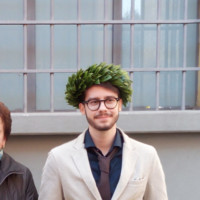
\includegraphics[width=0.2\textwidth]{../img/me.jpg}
	\hspace{8pt}
	\parbox[b]{5cm}{
	\metasection{Status:}{Undergraduate}
	\metasection{Lang:}{Java, C, C\#, Python, Scala, Assembler}
	\metasection{Data:}{SQL, MySQL, MongoDB}
	\metasection{WebDev:}{Angular, React, SCSS, HTML, CSS, PHP, Javascript, Bootstrap}
	\metasection{Tools:}{Git, Terminal, Eclipse, IntelliJ, Visual Studio, Spyder, Arduino IDE, Android Studio}
	}
}
\end{center}
\end{minipage}}\\[-4pt]

\fcolorbox{light}{light}{
\begin{minipage}[c][0.36\textheight][t]{\linewidth}
\vspace{4pt}
\hspace{26pt}
\parbox[c]{0.75\linewidth}{

\cvevent{nov - dec 2017}{LAMP Stack Back-end Developer}{Cosmobile S.R.L.}{Main activities and responsibilities: design and implementation of web-based software\\ 
$\>$ $\>$ on LAMP stacks based on a corporate framework derived from the Zend Framework\\
$\>$ $\>$ within the development team.}{Skills and objectives achieved: learning to analyze and design software, applying the\\
$\>$ $\>$ main design patterns. Learn to structure test plans.}

\cvevent{jul - aug 2013}{IT Assistance}{BE Infrastrutture S.R.L.}{Main activities and responsibilities: IT assistance both on-site and remotely for the staff\\
$\>$ $\>$ of the various CMC Ravenna offices. RDA and ORD data management. Created at the\\
$\>$ $\>$ request of the company a Java program for monitoring of servers' hard disks capacity.\\
$\>$ $\>$ Management of the corporate network alongside the company tutor.}{Skills and objectives achieved: Basic networking knowledge. Management and\\
$\>$ $\>$ resolution of IT issues. Design and development software.}

\cvevent{apr 2013}{IT Assistance}{BitLine sas}{Main activities and responsibilities: Computer assembly and repair, data entry and\\
$\>$ $\>$ management of the company website.}{Skills and objectives achieved: Learned business dynamics. Expanded knowledge\\
$\>$ $\>$ of computer hardware components.}

}
\hspace{18pt}
\textcolor{sectcol}{\rule[-3.2cm]{2pt}{7cm}}
\hspace{12pt}
\rotatebox[origin=c]{270}{\HUGE \textsc{Experience}}
\end{minipage}}\\[-4pt]

\fcolorbox{bgcol}{bgcol}{
\begin{minipage}[c][0.03\textheight][t]{\linewidth}
\vspace{-3pt}
\begin{center}
\parbox[b]{0.75\linewidth}{
	\begin{center}
	\large
	\textcolor{white}{Check out my open source projects at - } \textcolor{sectcol}{\textbf{\href{https://github.com/LorenzoChiana}{github.com/LorenzoChiana}}}
	\end{center}
}
\end{center}
\end{minipage}}\\[-4pt]

\fcolorbox{white}{white}{
\begin{minipage}[c][0.2875\textheight][t]{\linewidth}
\vspace{1pt}
\hspace{26pt}
\parbox[c]{0.75\linewidth}{

\cvevent{2018 - now}{Second Cycle Degree in Computer Science and Engineering}{UniBo}{Data knowledge engineering profile.}{Thesis title:}

\cvevent{2014 - 2017}{First Cycle Degree in Computer Science and Engineering}{UniBo}{During my university career, I developed several projects ranging from web development\\
$\>$ $\>$ to programming of embedded systems and IoT.}{Thesis title: \textit{``Ospedale 4.0: Sfide dell'IoT in ambito intra-ospedaliero"}}

\cvevent{2009 - 2014}{High School}{ITIS N. Baldini}{Graduated in computer science from the technical industrial institute Nullo Baldini}{Basic programming and networking knowledge}
}
\hspace{18pt}
\textcolor{sectcol}{\rule[-2.5cm]{2pt}{5.5cm}}
\hspace{12pt}
\rotatebox[origin=c]{270}{\HUGE \textsc{Education}}
\end{minipage}}\\[-4pt]


\fcolorbox{bgcol}{bgcol}{
\begin{minipage}[c][0.01\textheight][t]{\linewidth}
\vspace{-12pt}
\begin{center}
\parbox[b]{0.75\linewidth}{
	\begin{center}
	 \textcolor{white}{\href{www.lorenzochiana.com}{www.lorenzochiana.com}}
	\end{center}
}
\end{center}
\end{minipage}}
\end{document}